%!TEX root = main.tex

\section{Architectures}
Classical games like chess or tic-tac-toe are usually ``solved'' by AIs using a
single approach and searching through a single tree of game states, though
usually by optimizing the search and tree in various ways.

In comparison most approaches to AIs playing real-time strategy games usually
have to use domain knowledge do further subdivide the problem of playing the
game, because of the fine-grained simulations involved, and the various levels
of abstraction that is needed to get a successful AI. And especially when
approaching the way humans think about a problem more complex architectures
are needed.

\subsection{Decomposition of problem}
Michael Buro in his 2003 call for research \cite{buro2003real} identified six
important sub-problems in real-time strategy games that he said would be
interesting for AI research to focus on. These problems also dictates how the architecture has to e structured in order to solve them. It is therefor important to have a clear view of what the different main sub-problems are and how they will affect each other.

\begin{description}
  \item [Resource management.] Resources are what is used to create buildings and units. There are four main things one can spend resources on in starcraft, that is creating new buildings, researching upgrades, expanding to new bases and producing units. In order to be an efficient player one has to find a good balance between all four of these, and perform the right action at the right time. Like allocating more money for units and defenses if one is under attack. Resource management is a big part of the macro play, and making sure to always spend the resources efficient will be very important for any starcraft bot.
  \item [Decision making with uncertainty.] Because fog of war hides all the parts of the map where the player have no units, there is a
    high degree of uncertainty involved in the decision making. Scouting then becomes essential, as the more information you can gather about the enemies activities the less uncertainty you have to work with. To deal with uncertainty the AI needs to create hypotheses about the enemies strategies, and then act according to them. It should also it should scout to confirm these hypotheses.
  \item [Spatial and temporal reasoning.] Spatial and temporal reasoning is a huge part of any military simulator. Identifying choke points and predicting outcomes and
    utilities of actions it takes are some obvious applications.
  \item [Collaboration.] In most RTSes it is possible for players to ally, and
    how to share intelligence and coordinate attacks is a challenging problem,
    though maybe not as interesting yet.
  \item [Opponent modelling.] Learning from the opponent is an important skill,
    and exploting the weaknesses of your opponent is an important aspect of
    human-level playing.
  \item [Adverserial real-time planning.] Abstracting away micro-level
    management to allow for more efficient search in the game state-space, and
    translate the found solutions back, is an important problem to solve.
\end{description}

A lot of research as been done into AIs for RTSes since this, however, and the
list might be a bit outdated. For example, one important aspect of most AIs
today is the micro-management of units, trying to maximize the utility of them 
(maximizing output of resource gatherers and damage dealt by offensive units,
for example).

Another important problem that is under-valued by the above list is learning
from existing knowledge, like learning build-orders from replays of games played
by humans (or other bots, though the utility of that might not be substantial).
This can be integrated into several of the items above, for example the decision
with uncertainty by statistically inferring the most probable states by
learning from earlier games.

A more general and simplified breakdown of the problem of playing Starcraft can
be found in Ben Weber's presentation from the AIIDE 2010 StarCraft AI
Competition:\cite{weber2010aiide}

\begin{description}
  \item [Managing economy] is the same as the resource management mentioned
    above, and is about getting a steady income.
  \item [Expanding the tech tree] to get more powerful and varied units.
  \item [Producing units] is perhaps one of the most complex parts. This
    involves both buildings and movable units, defensive and offensive.
  \item [Attack opponent] usually is not a very explicit action, but can still
    be pretty complex, since one needs to evaluate its own state against what
    it knows about the opponent to know when to attack, and where. This point
    also involves micro-management, which has received a lot of attention from 
    authors of AIs that have ranked highly.
\end{description}

Solving all of the aforementioned problems by themselves are what is the focus
of most research today, but another important problem is tying all of these
solutions together again. This is perhaps one of the most basic, but important,
aspects of the architecture. There are several different ways of doing this,
and some of the most common one is simply sharing a large amount of information
between sub-units in the architecture (for example a black-board based
architecture), or simply having a well-defined graph hierarchy where decisions
are propagated.

\subsection{Architectures of current state of the art Starcraft AI}
Each year there are several big AI conferences that run Starcraft AI RTS competitions. The the two biggest are held at the Computational Intelligence in Games conference(CIG)\footnote{\url{ttp://ls11-www.cs.uni-dortmund.de/rts-competition/starcraft-cig2011}} and the AI and interactive digital entertainment conference(AIIDE)\footnote{\url{http://www.starcraftaicompetition.com/}}. Here most the the state of the art bots come together to measure their strength compared to the other bots. Most of the time playing vs a real player is not something that the bots can be very effective, so these competitions becomes the only real way for researchers and developers to test their AIs and get some reasonable feedback on the level of play they are capable of.

\subsubsection{BTHAI}
BTHAI utilizes a multi-agent approach to create a system with high levels of modularity. Each unit and building is represented as an agent that extends a more general version of that agent type. So every building is a subclass of a structurAgent, and every unit is a subclass of an unitAgent. These again extend a baseAgent, and this creates a hierarchic structure where agents of a similar type can share logic for behavior and strategy, but supports the option of extending the agent in order to customize and specialize the behavior of that specific agent. 

For higher level tasks with as tactics, exploration and building the bot uses managers. The managers maintains all the agent objects for the different units that the bot controls. Managers also act as an information provider for the agents so they can access data and statistics about the current state of the game. For instance how many units that an attacking force consists of, and how many are defending the base etc. 
There are also an exploration manager, that handles everything related to exploration, where enemy units have been discovered and predictions about where they will move. A build planer decides what order buildings will be constructed in, and squad commanders handles higher level tactics for a group of units, like attacking or retreating. These managers also have an hierarchic structure, so that they can be extended in order to create a more specialized manager, like a race specific build planer. 

The creation of agent instances are the responsibility of an AgentFactory. This factory makes sure that the correct agent is created for a given unit and that if there exists a specialized agent type for that unit the correct one is created and not a general agent. 

For movement of individual units the bot utilizes a potential field implementation. Agents can decide depending on the situation and the need for precise movements if they want to use the built-in starcraft path-finding or the potential field module. 

Figure \ref{fig:bthaiarch} shows a general overview of the architecture used in BTHAI

% TODO: maybe clear page here if that fits when report is done. 

\begin{figure}[h!tbp]
\centering
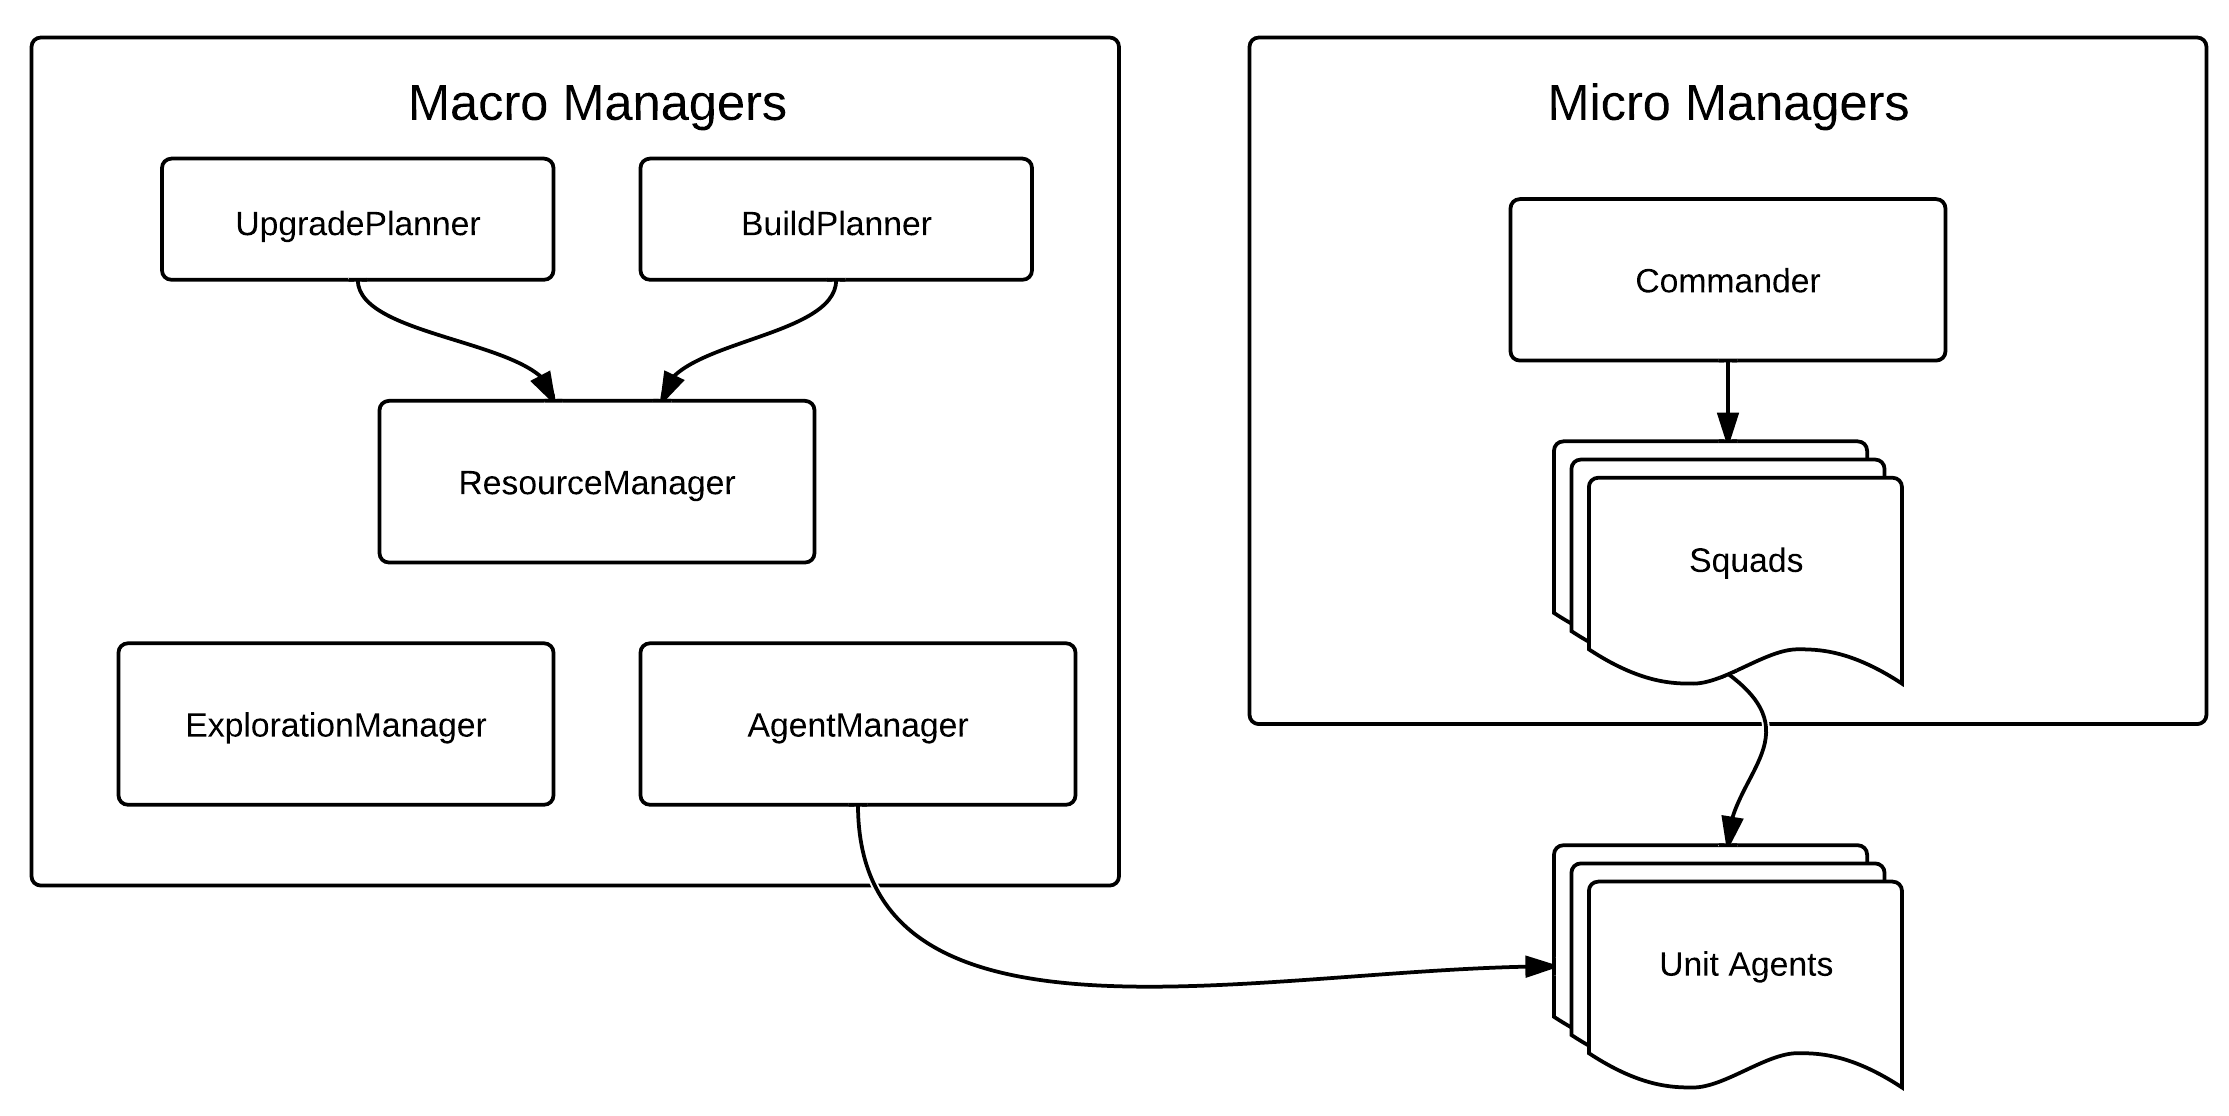
\includegraphics[scale=0.8]{graphics/bthai.png}
\caption{BTHAI general architecture}
\label{fig:bthaiarch}
\end{figure}

\subsubsection{BroodwarBotQ}
BroodwarBotQ has taken a more divide-and-conquer approach to the higher levels of macro control then BTHAI. Meaning it has separate agent types for the different tasks that a starcraft game consists of. Worker manager, bases manager, production manager, and construction manager are some of the macro oriented agent types that this bot utilizes. None of the managers controls are orders any of the others around, so the problem of playing starcraft is divided into subtasks that each has a manager that should solve them. But some of the subtasks are not entirely independent, so in order to resolve conflicts between the modules BroodwarBotQ uses a arbitrator. This also acts as a mediator between the macro and micro layers of the architecture. 

For this bot unit control is realized using Bayesian units that strives for completion different goals as ordered by an goal manager.\cite{synnaeve2011bayesian} One of the main goals for the author of BroodwarBotQ was improve the intelligence of starcraft bot, mainly the ability to predict and change strategy based on what the opponent is planing. So achieve this they have estimators that based on data extracted from starcraft replays using Bayesian models, tries to predict what the opponent are doing and planing and tries to adapt its own game play according to countering that. 

% TODO: maybe clear page here if that fits when report is done. 

\begin{figure}[h!tbp]
\centering
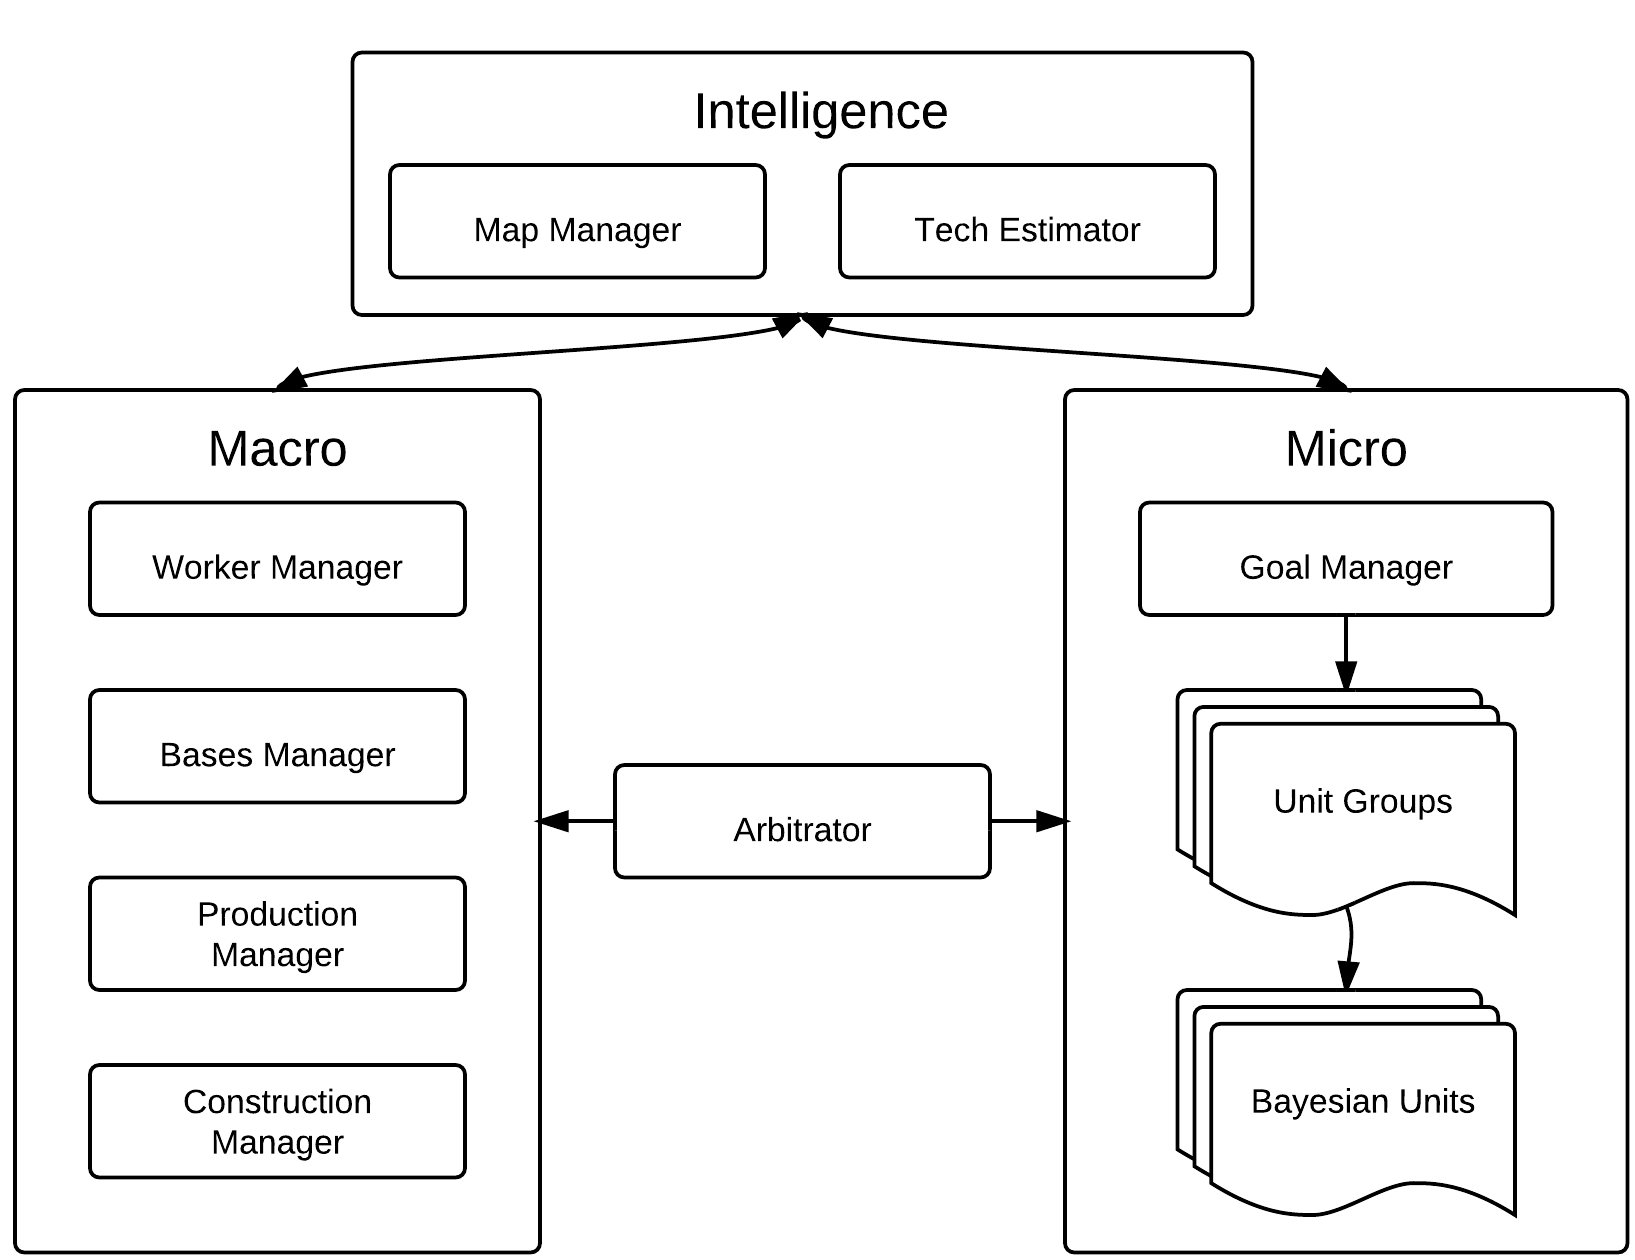
\includegraphics[scale=0.8]{graphics/bbq.png}
\caption{BroodwarBotQ general architecture}
\label{fig:bbqarch}
\end{figure}

\subsubsection{Skynet}
Skynet uses a more hierarchic approach then most of the other bots, where it has divided its decision making into three different layers. Where higher level modules issuing commands to the lower level modules. The strategy layer at the top manages build order strategies that it gives commands to the tactics layer underneath to execute. The tactics layer contains all the managers that controls all the different aspects of the game, like resource management, scouting and macro management. All this managers outputs tasks that have to be completed and sends them to the task manager in the last layer. In this task layer each of the tasks in the queue will be given to a specific low level module that knows how to execute it. This is the only place where commands are sent from the bot to Starcraft. In addition the bot has a series of situational analysis modules that that continuously analyses the state of the game, and gives input back to the decision making layers when it identifies something that needs focus.

% TODO: maybe clear page here if that fits when report is done. 

\begin{figure}[h!tbp]
\centering
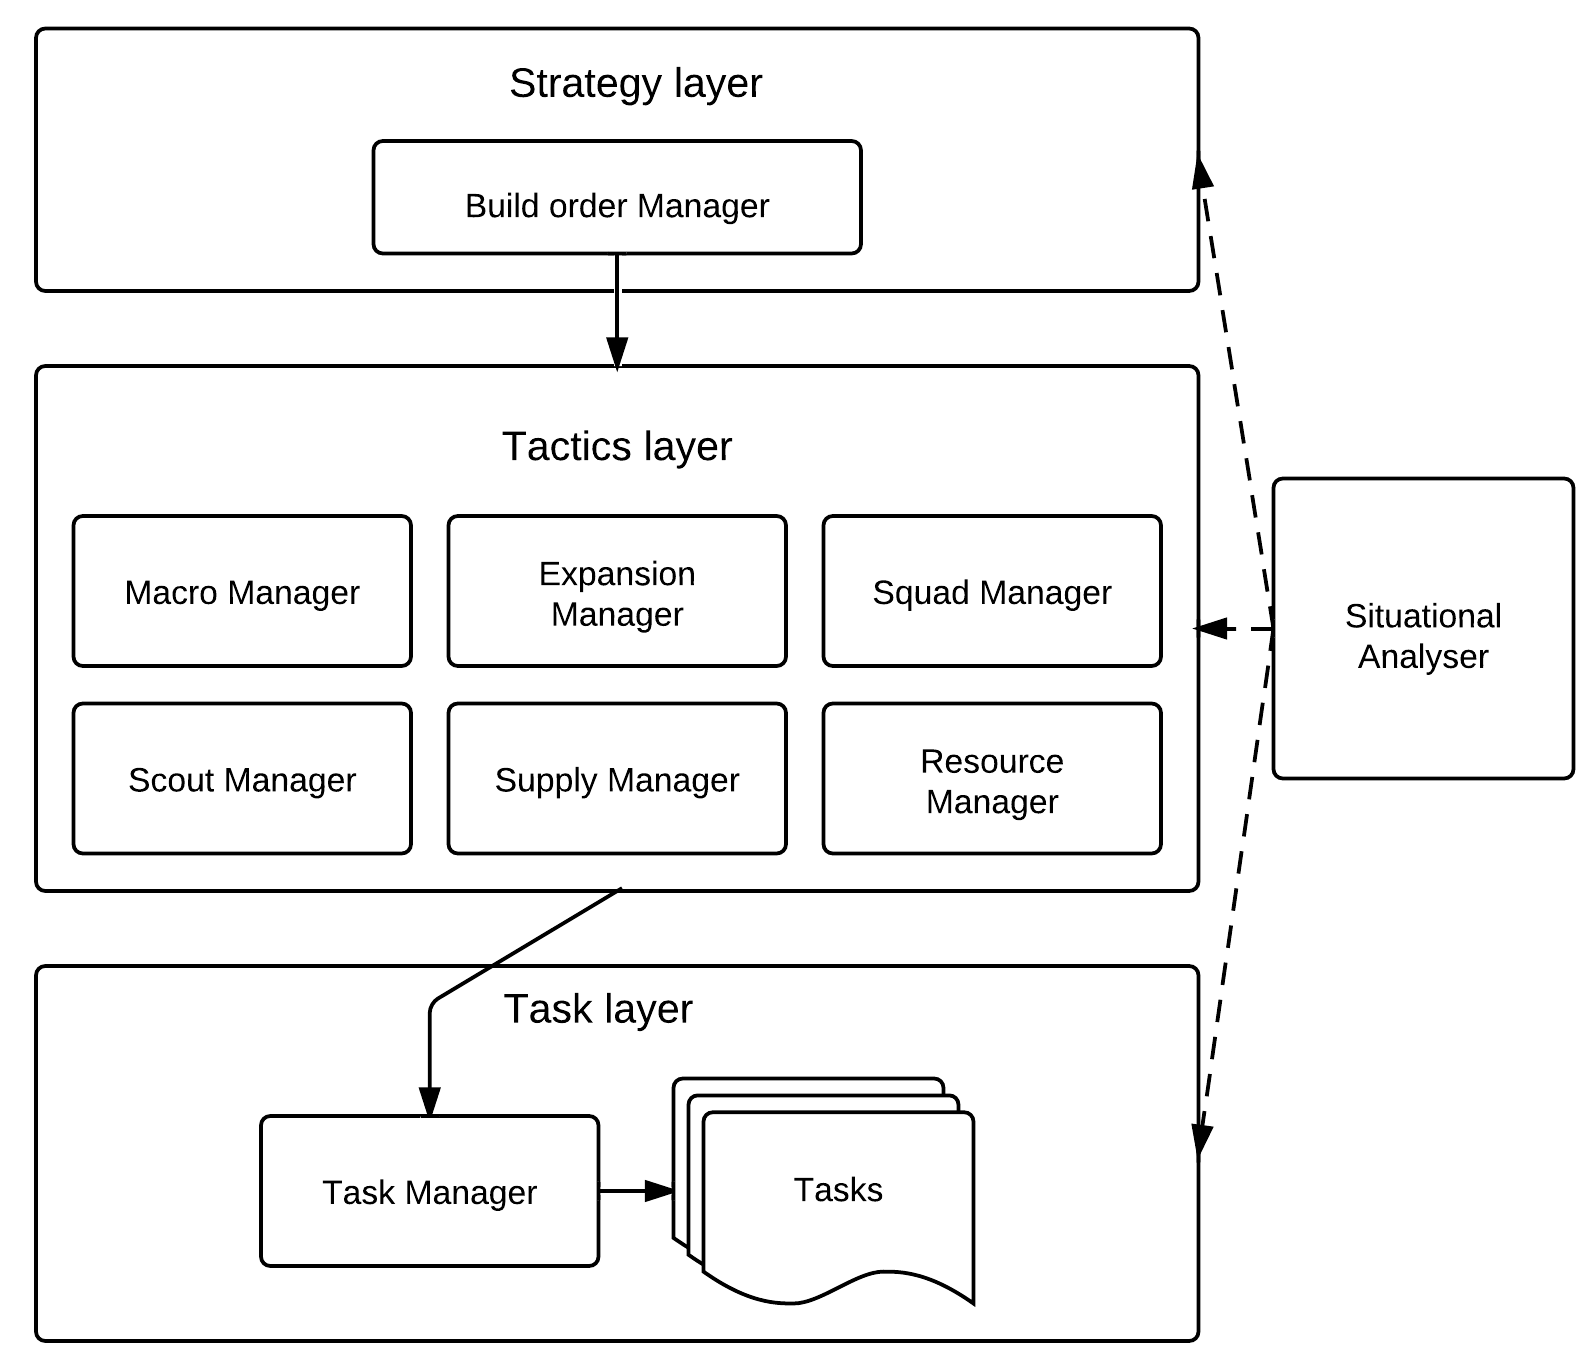
\includegraphics[scale=0.8]{graphics/skynet.png}
\caption{Skynet general architecture}
\label{fig:skynetarch}
\end{figure}

\subsubsection{Nova}
Nova\cite{pérezmulti} has an architecture design that is quite close to BroodwarBotQ, except it uses a blackboard instead of an arbitrator. Nova is designed as a multi-agent system with managers and agents, and was design with that idea that having maximum possible information about the enemy at all times is essential for creating a good AI. Micro management is handled by abstraction, meaning you have a hierarchic system with general agents and the top, like the squad agent that is in charge of controlling an entire squad of units, and more specific agents at the bottom, like the Combat agent that handles fighting for the individual unit on the battlefield. Where as macro is handled with divide-and-conquer where a big problem is divided into smaller individual problems that each have a manager that tries to solve it. 

To achieve the initial goal of maximum information access the bot uses a blackboard for communication. Here all the modules can post data and intentions, and the other modules can then read this data. Anyone can read and write here, and all the information is available to every module that wants it. 

% TODO: maybe clear page here if that fits when report is done. 

\begin{figure}[h!tbp]
\centering
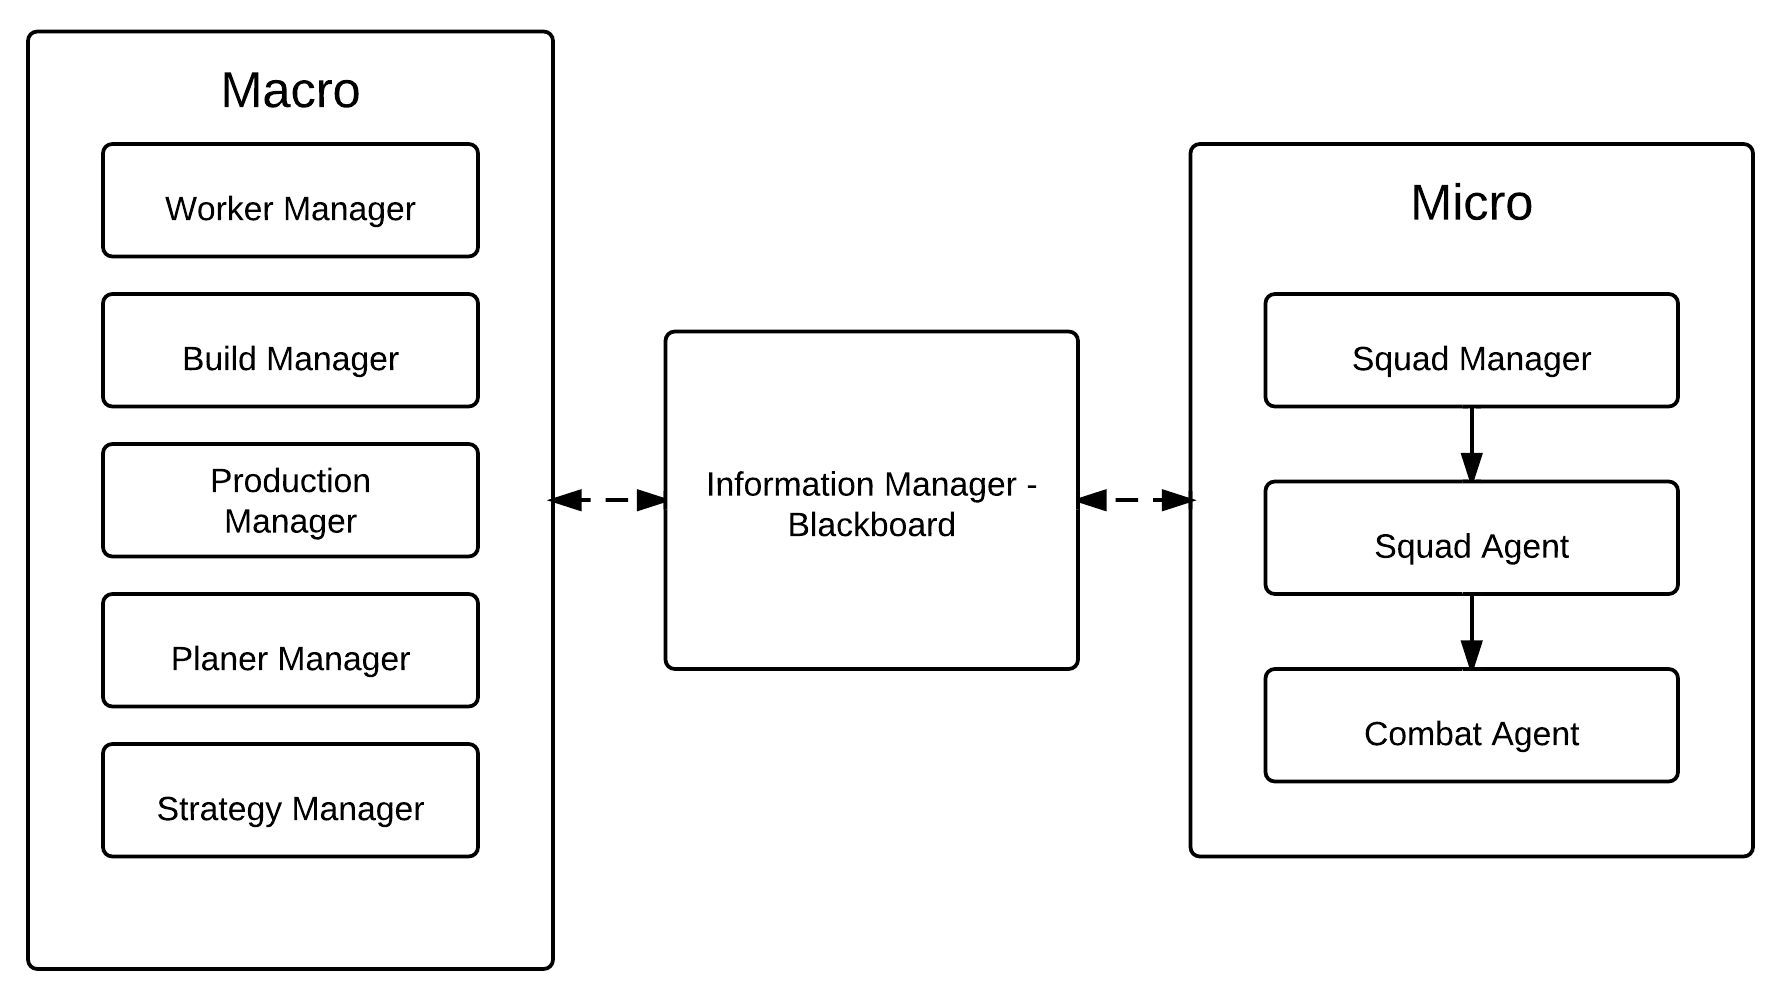
\includegraphics[scale=0.8]{graphics/nova.png}
\caption{Nova general architecture}
\label{fig:novaarch}
\end{figure}

